%TODO cambiare la foto
\begin{figure}[H]
  \centering
    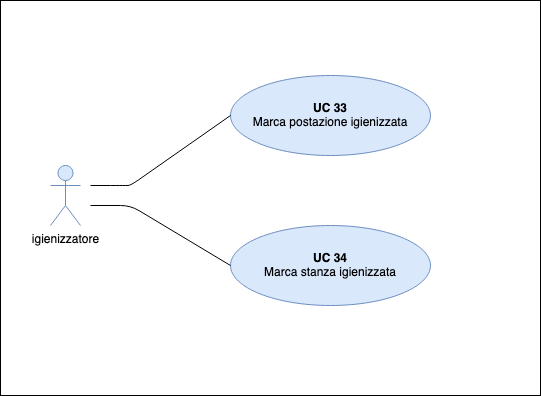
\includegraphics[width=\textwidth]{src/CasiDUso/immagini/UC-igienizzazionePostazioni.png}
  \caption{Igienizzazione postazioni}
\end{figure}

%TODO modificare su Web la registrazione di un nuovo utente aggiungendo il flag per amministratore o igienizzatore
\subsection{UC- Marca stanza igienizzata}

\begin{itemize}
\item \textbf{Attori primari:} igienizzatore;
\item \textbf{Descrizione:} l’igienizzatore può marcare un'intera stanza come igienizzata, pertanto ogni postazione al suo interno è sanificata e servibile quindi dagli utenti;
\item \textbf{Precondizione:} l'igienizzatore naviga nell’apposita sezione di igienizzazione della stanza; 
\item \textbf{Postcondizione:} l'igienizzatore ha marcato con successo una stanza come igienizzata;
\item \textbf{Scenario principale:} 
	\begin{itemize}
		\item l'igienizzatore seleziona la stanza da marcare come igienizzata;	
		\item l'igienizzatore contrassegna la stanza come igienizzata;
		\item il sistema elabora correttamente la richiesta contrassegnando tutte le postazioni all'interno della stanza come igienizzate.
		\end{itemize}
\end{itemize}

\subsection{UC- Visualizzazione stanze da igienizzare}

\begin{itemize}
\item \textbf{Attori primari:} igienizzatore;
\item \textbf{Descrizione:} l’igienizzatore può visualizzare l'elenco delle stanze (contrassegnate dal nome univoco) da igienizzare;
\item \textbf{Precondizione:} l'igienizzatore si trova nell’apposita sezione di visualizzazione delle stanze da igienizzare; 
\item \textbf{Postcondizione:} l'igienizzatore ha ricevuto l'elenco delle stanze da igienizzare;
\item \textbf{Scenario principale:} 
	\begin{itemize}
		\item il sistema elabora la richiesta;
		\item il sistema restituisce la lista delle stanze da igienizzare;
		\end{itemize}
\end{itemize}



%TODO DESIDERABILE (se non hai gli strumenti per pulire)
%\subsubsection{UC-43 - Marca stanza non igienizzata}

%\begin{itemize}
%\item \textbf{Attori primari:} igienizzatore;
%\item \textbf{Descrizione:} l’igienizzatore può annullare lo stato di stanza igienizzata precedentemente segnato, impostando la stanza come “non igienizzata”;
%\item \textbf{Precondizione:} l'utente naviga nell’apposita sezione di gestione della stanza; 
%\item \textbf{Postcondizione:} l'utente ha marcato con successo una stanza come non igienizzata;
%\item \textbf{Scenario principale:} 
%	\begin{itemize}
%		\item l’utente naviga nell’apposita sezione di gestione della stanza;	
%		\item l'utente contrassegna la stanza come non igienizzata;
%		\item il sistema elabora correttamente la richiesta;
%	\end{itemize}
%\end{itemize}
